\documentclass[journal,onecolumn]{IEEEtran}
\usepackage{header}

\usepackage[portuguese]{babel}
% \usepackage[backend=biber]{biblatex}
% \addbibresource{references.bib}

\title{
    TP4: Análise Quantitativa do Trade-off entre Especialização e Generalização em LLMs via Fine-Tuning
}

\author[1]{Lucas Castro de Souza \thanks{lucas.castro@icomp.ufam.edu.br}}
\affil[1]{Universidade Federal do Amazonas - PPGI}

\newcommand{\figwidth}{0.7\linewidth}

\begin{document}

\maketitle
\IEEEpeerreviewmaketitle

%1. Objetivo
% O objetivo central deste projeto é a avaliação empírica e sistemática do processo de fine-tuning em Modelos de Linguagem de Grande Porte (LLMs).
% Os alunos irão implementar, treinar e avaliar um LLM para a tarefa de Text-to-SQL. A análise quantificará o ganho de desempenho na tarefa-alvo e,
% simultaneamente, medirá a degradação de performance em tarefas de conhecimento geral. O projeto exige a implementação de métricas de
% avaliação customizadas e uma análise crítica dos trade-offs inerentes à especialização de modelos.
% 2. Problema
% A especialização de LLMs via fine-tuning é uma técnica proposta para otimizar o desempenho em domínios específicos. Contudo, este
% processo de otimização focado pode comprometer a robustez do modelo em tarefas que não pertencem ao domínio de treinamento, um
% fenômeno conhecido como "esquecimento catastrófico" ou "regressão de capacidade". Esse trabalho consiste em projetar e executar
% um pipeline experimental que permita medir com precisão ambas as facetas deste fenômeno: o ganho de especialização e a perda de
% generalização.
% 3. Materiais e Configuração
% ● Modelo Base: Deve ser utilizado um modelo open-source da classe de 7-8 bilhões de parâmetros em sua versão instruct/chat. Modelos
% sugeridos: meta-llama/Llama-3-8B-Instruct, mistralai/Mistral-7B-Instruct-v0.2. A versão exata do checkpoint utilizado
% deve ser documentada para garantir a reprodutibilidade.
% ● Dataset de Fine-Tuning: Spider Dataset, disponível no site oficial. Utilizar exclusivamente o training split. Os dados devem ser
% pré-processados para o formato exigido pelo framework de treinamento escolhido (e.g., formato de chat com [INST], [SYS]).
% ● Dataset de Avaliação de Tarefa: Spider development split. Este conjunto de dados não deve ser visto pelo modelo durante o treinamento.
% ● Dataset de Avaliação de Generalização: MMLU (Massive Multitask Language Understanding), disponível no Hugging Face Hub. Deve ser
% criada uma suíte de avaliação composta por exatamente 150 questões, divididas igualmente em 3 categorias:
% 1. STEM: 50 questões de uma subcategoria (e.g., computer_science).
% 2. Humanidades: 50 questões de uma subcategoria (e.g., philosophy).
% 3. Ciências Sociais: 50 questões de uma subcategoria (e.g., economics).
% ● Framework de Avaliação: DeepEval (versão 0.21.x ou superior).
% ● Frameworks de Treinamento: Hugging Face TRL, Axolotl ou similar

\section{Observações}
Algumas observações importantes sobre o trabalho:
\begin{itemize}
    \item O repositório com o código do trabalho está disponível em \url{https://github.com/lcs147/nlp-tp4}.
    \item Os checkpoints do LoRA e os resultados intermediários estão disponíveis em \href{https://drive.google.com/drive/folders/1VXzIdSLtCn5-leHEG6usvXw60Y5OzKKv?usp=sharing}{Link}.
    \item O parâmetro variado no experimento foi o número de épocas de fine-tuning. Foram avaliados o modelo base (sem fine-tuning), o modelo fine-tuned por 3 épocas e o modelo fine-tuned por 5 épocas.
    \item O modelo foi fine-tunado utilizando o dev split do Spider. Eu só percebi após finalizar que a especificação pedia o train split.
    \item Para a avaliação na tarefa de Text-to-SQL, utilizei apenas as 150 primeiras instâncias do Spider dev split. Isso ocorreu porque eu estava na terceira (e última) conta do Colab e não seria possível avaliar todas as $1034$ instâncias. Para executar com todas as instâncias, basta alterar o valor da variável EVALUATION\_ENTRIES\_SIZE em $common.py$ para $1034$.
\end{itemize}

\section{Metodologia}
 A seguir, está detalhada cada etapa do pipeline experimental deste trabalho, incluindo arquitetura dos scripts, o pré-processamento dos dados, configuração do modelo base, a configuração do treinamento com LoRA, e a implementação da métrica customizada de avaliação.

\subsection{Arquitetura dos Scripts}

O projeto foi organizado em seis scripts principais. Cada um é responsável por uma etapa específica do pipeline experimental, eles foram executados na mesma ordem em que são apresentados aqui. A seguir, uma breve descrição de cada script:

\begin{itemize}
    \item \textbf{0\_preparando\_dados.py}: Responsável pelo pré-processamento dos dados. Este script carrega o Spider dataset, extrai e formata os exemplos para o formato de chat utilizado no fine-tuning e avaliação. Também prepara e salva o conjunto de questões do MMLU, garantindo a divisão correta por categorias.

    \item \textbf{1\_fine-tuning.py}: Realiza o treinamento supervisionado do modelo base utilizando LoRA. Implementa o pipeline de tokenização, configuração dos hiperparâmetros do LoRA, argumentos de treinamento e execução do processo de fine-tuning, salvando checkpoints intermediários.

    \item \textbf{2\_calculando\_baseline.py}: Calcula o desempenho de baseline do modelo base (sem fine-tuning) na tarefa de Text-to-SQL. Utiliza exemplos 3-shot e executa as queries geradas, comparando com as respostas de referência para medir a acurácia inicial.

    \item \textbf{3\_avaliacao\_customizada.py}: Avalia os modelos fine-tuned utilizando a métrica customizada \textit{ExecutionAccuracy} utilizando o framework DeepEval. Gera prompts, executa as queries SQL produzidas pelo modelo e compara os resultados com o ground truth, salvando checkpoints e resultados detalhados.

    \item \textbf{4\_analise\_mmlu.py}: Mede a generalização dos modelos (base e fine-tuned) no benchmark MMLU. Gera prompts 4-shot para questões de múltipla escolha, executa a inferência e calcula métricas de acurácia e desvio padrão por categoria.
\end{itemize}

Para garantir a reprodutibilidade dos experimentos, todos os seeds dos geradores de números aleatórios foram fixados em 42. Sempre que possível, opções determinísticas foram selecionadas nos frameworks utilizados para minimizar variações entre execuções.

\subsection{Pré-processamento dos Dados}
O pré-processamento dos dados é necessário para garantir a compatibilidade dos datasets com o modelo e os frameworks utilizados. Inicialmente, o Spider dataset foi carregado a partir do arquivo original \texttt{dev.json}. Para cada entrada, foi extraída a questão em linguagem natural, a query SQL de referência e o esquema do banco de dados correspondente. O esquema foi reconstruído em formato textual, listando todas as tabelas e colunas presentes no banco, de modo a fornecer ao modelo o contexto necessário para a geração da query. Veja a Figura~\ref{fig:spider_processed} para um exemplo de entrada do Spider dataset após o pré-processamento.

\begin{figure}[!htpb]
    \centering
    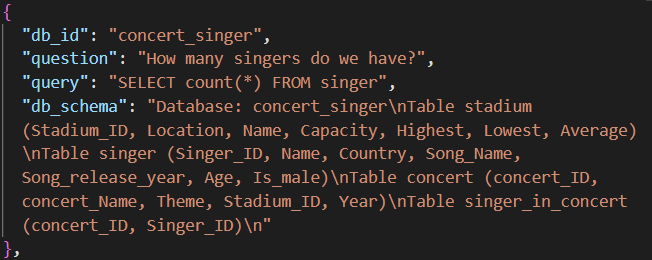
\includegraphics[width=\figwidth]{resources/spider_processed.png}
    \caption{Exemplo de entrada do Spider dataset após pré-processamento}
    \label{fig:spider_processed}
\end{figure}

Cada exemplo foi então convertido para o formato de chat, seguindo o padrão de prompts utilizado por modelos da família Qwen. O prompt inclui um bloco \texttt{system} com a instrução geral, um bloco \texttt{user} contendo o esquema do banco e a questão, e um bloco \texttt{assistant} com a query SQL de referência (no caso do treinamento) ou vazio (no caso da inferência). A Figura~\ref{fig:spider_prompt} ilustra a função que cria o prompt de inferência para uma consulta do Spider.

\begin{figure}[!htpb]
    \centering
    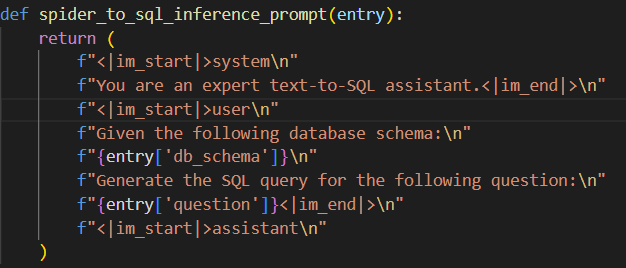
\includegraphics[width=\figwidth]{resources/spider_prompt.png}
    \caption{Função que cria um prompt de inferência para uma consulta do Spider.}
    \label{fig:spider_prompt}
\end{figure}

Para a avaliação de generalização, foi utilizada uma amostra de 150 questões do benchmark MMLU, divididas igualmente entre as categorias STEM (elementary\_mathematics), Humanidades (philosophy) e Ciências Sociais (management). As questões foram selecionadas de subcategorias específicas e processadas para o formato de prompt compatível, incluindo o enunciado da questão e as alternativas de resposta. A Figura~\ref{fig:mmlu_processed} ilustra o formato de uma questão do MMLU após o processamento.
\begin{figure}[!htpb]
    \centering
    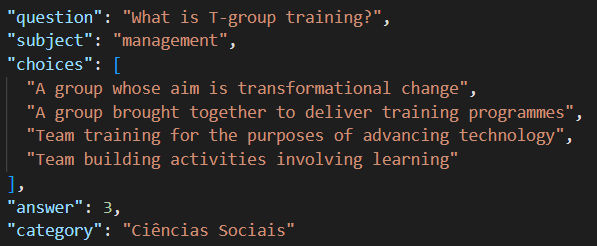
\includegraphics[width=\figwidth]{resources/mmlu_processed.png}
    \caption{Formato de uma questão do MMLU após ser processada.}
    \label{fig:mmlu_processed}
\end{figure}

\subsection{Configuração do Modelo Base}

O modelo base utilizado neste experimento foi o \texttt{Qwen/Qwen2-7B-Instruct}. A escolha deste modelo se deve a ser um modelo de 7 bilhões de parametros e ter boa performance no benchmark MMLU-Pro.

Ele foi carregado de forma quantizada pois ele não cabe sem quantização na GPU grátis do Google Colab (T4 15GB), que foi utilizada para o treinamento e avaliação. Foi utilizado também, \texttt{float16} pois a GPU grátis do Google Colab não suporta \texttt{bfloat16}. Veja Figura~\ref{fig:base_model_config} para detalhes da configuração de carregamento do modelo.

\begin{figure}[!htpb]
    \centering
    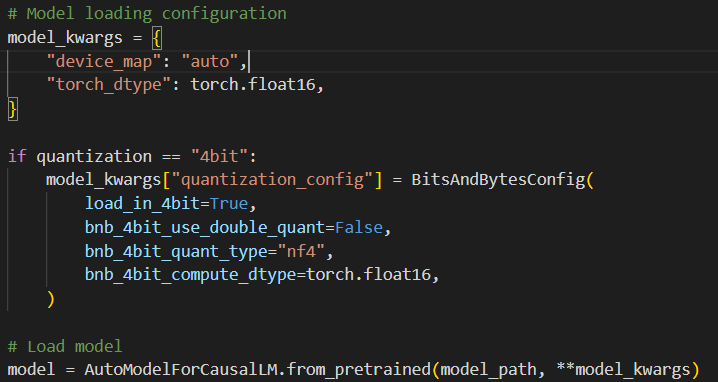
\includegraphics[width=\figwidth]{resources/base_model_config.png}
    \caption{Configuração de carregamento do modelo em modo quantizado.}
    \label{fig:base_model_config}
\end{figure}


\subsection{Configuração do Treinamento com QLoRA}

O fine-tuning foi realizado utilizando o método QLoRA (Quantized Low-Rank Adaptation). Foram adaptados apenas os módulos de atenção do modelo (\texttt{q\_proj}, \texttt{k\_proj}, \texttt{v\_proj}, \texttt{o\_proj}), reduzindo o número de parâmetros treináveis e acelerando o processo de fine-tuning. A configuração do LoRA adotada está detalhada na Figura~\ref{fig:lora_config}.

\begin{figure}[!htpb]
    \centering
    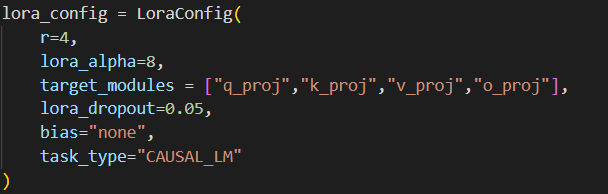
\includegraphics[width=\figwidth]{resources/lora_config.png}
    \caption{Configuração LoRA.}
    \label{fig:lora_config}
\end{figure}

\subsection{Configuração do Treinamento}

O treinamento foi conduzido por 5 épocas, com batch size efetivo de 8 (batch size 2 e \textit{gradient accumulation steps} 4), taxa de aprendizado inicial de $2 \times 10^{-4}$, otimizador AdamW em modo 8-bit.

Os checkpoints do LoRA foram salvos a cada época para permitir a avaliação do finetuning em diferentes épocas, como pedido na especificação do trabalho. Veja a Figura~\ref{fig:training_config} para detalhes da configuração do treinamento.

\begin{figure}[!htpb]
    \centering
    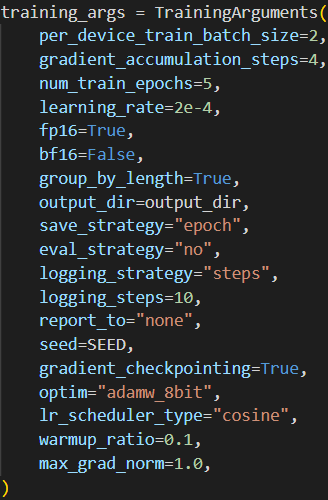
\includegraphics[width=0.25\linewidth]{resources/training_config.png}
    \caption{Configuração do Treinamento.}
    \label{fig:training_config}
\end{figure}

\subsection{Implementação da Métrica Customizada: ExecutionAccuracy}

Para avaliar a geração de consultas SQL, foi implementada a métrica customizada \textbf{ExecutionAccuracy}, compatível com o framework DeepEval. Essa métrica executa tanto a query gerada pelo modelo quanto a de referência no mesmo banco SQLite, atribuindo score 1.0 se os resultados coincidirem (ignorando ordem e duplicatas) e 0.0 caso contrário ou em caso de erro de execução. Mensagens de erro são registradas para análise posterior. A Figura~\ref{fig:custom_metric_main} mostra o núcleo da implementação.
\begin{figure}[!htpb]
    \centering
    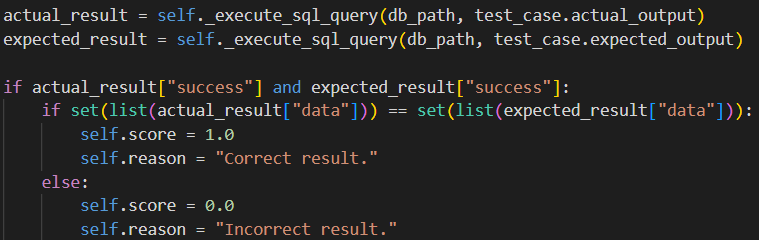
\includegraphics[width=\figwidth]{resources/custom_metric_main.png}
    \caption{Parte principal da função que avalia os resultados.}
    \label{fig:custom_metric_main}
\end{figure}

% add new figure
\section{Resultados}
% Os resultados devem ser apresentados com clareza estatística (e.g., médias, desvio padrão). É fortemente recomendada a inclusão de uma breve análise de erros, examinando 2-3 exemplos onde o modelo fine-tuned falhou na tarefa-alvo.
\subsection{Desempenho na Tarefa Text-to-SQL (Spider)}

A Tabela~\ref{tab:spider_results} apresenta as acurácias médias e desvios padrão dos modelos avaliados na tarefa de Text-to-SQL, considerando as 150 primeiras instâncias do Spider dev split.

\begin{table}[h]
\centering
\caption{Resultados na tarefa Spider (Text-to-SQL)}
\label{tab:spider_results}
\begin{tabular}{lccc}
\toprule
\textbf{Modelo} & \textbf{Épocas} & \textbf{Acurácia} & \textbf{Desvio Padrão} \\
\midrule
Qwen2-7B-Instruct (base) & 0 & 0.480 & 0.501 \\
Qwen2-7B-Instruct-LoRA & 3 & 0.793 & 0.406 \\
Qwen2-7B-Instruct-LoRA & 5 & 0.907 & 0.292 \\
\bottomrule
\end{tabular}
\end{table}

A variação percentual de acurácia entre o modelo base e o modelo fine-tuned por 5 épocas foi de:
\[
\Delta_{\text{acurácia}} = \frac{0.907 - 0.480}{0.480} \times 100 \approx 89.0\%
\]
Ou seja, o \textbf{fine-tuning proporcionou um aumento de aproximadamente 89\% na acurácia na tarefa-alvo}.

\subsection{Desempenho em Generalização (MMLU)}

A Tabela~\ref{tab:mmlu_results} apresenta os resultados agregados e por categoria no benchmark MMLU, incluindo acurácia média e desvio padrão.

\begin{table}[h]
\centering
\caption{Resultados no MMLU (generalização por categoria)}
\label{tab:mmlu_results}
\begin{tabular}{lcccc}
\toprule
\textbf{Modelo} & \textbf{Agregada} & \textbf{STEM} & \textbf{Ciências Sociais} & \textbf{Humanidades} \\
\midrule
Base & 0.300 $\pm$ 0.016 & 0.320 $\pm$ 0.466 & 0.280 $\pm$ 0.449 & 0.300 $\pm$ 0.458 \\
LoRA (3 épocas) & 0.373 $\pm$ 0.038 & 0.400 $\pm$ 0.490 & 0.400 $\pm$ 0.490 & 0.320 $\pm$ 0.466 \\
LoRA (5 épocas) & 0.393 $\pm$ 0.057 & 0.460 $\pm$ 0.498 & 0.400 $\pm$ 0.490 & 0.320 $\pm$ 0.466 \\
\bottomrule
\end{tabular}
\end{table}

A variação percentual de acurácia agregada entre o modelo base e o modelo fine-tuned por 5 épocas foi de:
\[
\Delta_{\text{acurácia, MMLU}} = \frac{0.393 - 0.300}{0.300} \times 100 \approx 31.0\%
\]
Ou seja, \textbf{houve um aumento de aproximadamente 31\% na acurácia agregada no MMLU após o fine-tuning}.

A Tabela~\ref{tab:mmlu_delta} detalha a variação percentual por categoria:

\begin{table}[h]
\centering
\caption{Variação percentual de acurácia por categoria (MMLU, base $\rightarrow$ LoRA 5 épocas)}
\label{tab:mmlu_delta}
\begin{tabular}{lccc}
\toprule
\textbf{Categoria} & \textbf{Base} & \textbf{LoRA 5 épocas} & \textbf{Variação (\%)} \\
\midrule
STEM & 0.320 & 0.460 & $+43.8\%$ \\
Ciências Sociais & 0.280 & 0.400 & $+42.9\%$ \\
Humanidades & 0.300 & 0.320 & $+6.7\%$ \\
\bottomrule
\end{tabular}
\end{table}

Observa-se que o ganho de acurácia foi mais expressivo nas categorias STEM e Ciências Sociais, enquanto em Humanidades o aumento foi modesto.

\subsection{Análise de Erros}

Apesar do aumento significativo de desempenho, o modelo fine-tuned ainda apresenta falhas em alguns casos. A seguir, foram destacados dois exemplos de erro do modelo após 5 épocas de fine-tuning na tarefa Text-to-SQL:

\begin{itemize}
    \item \textbf{Input:} What is the count of the car models produced in the United States?\\
        \textbf{Output gerado:}
        \begin{flushleft}
        \texttt{SELECT count(*) FROM CAR\_MAKERS AS T1 JOIN COUNTRIES AS T2 ON T1.Country  =  T2.CountryId WHERE T2.CountryName  =  'United States'}
        \end{flushleft}
        \textbf{Output esperado:}
        \begin{flushleft}
        \texttt{SELECT count(*) FROM MODEL\_LIST AS T1 JOIN CAR\_MAKERS AS T2 ON T1.Maker  =  T2.Id JOIN COUNTRIES AS T3 ON T2.Country  =  T3.CountryId WHERE T3.CountryName  =  'usa';}
        \end{flushleft}

    \item \textbf{Input:} Which countries in europe have at least 3 car manufacturers?\\
        \textbf{Output gerado:}
        \begin{flushleft}
        \texttt{SELECT T1.CountryName FROM COUNTRIES AS T1 JOIN CONTINENTS AS T2 ON T1.Continent  =  T2.ContId JOIN CAR\_MAKERS AS T3 ON T1.CountryId  =  T3.Country WHERE T2.Continent  =  'Europe' GROUP BY T1.CountryName HAVING COUNT(*)  $\geq$  3;}
        \end{flushleft}
        \textbf{Output esperado:}
        \begin{flushleft}
        \texttt{SELECT T1.CountryName FROM COUNTRIES AS T1 JOIN CONTINENTS AS T2 ON T1.Continent  =  T2.ContId JOIN CAR\_MAKERS AS T3 ON T1.CountryId  =  T3.Country WHERE T2.Continent  =  'europe' GROUP BY T1.CountryName HAVING count(*)  $\geq$  3;}
        \end{flushleft}
\end{itemize}
Nestes exemplos, o modelo errou ao utilizar valores incorretos para os nomes de países ('United States' vs 'usa' e 'Europe' vs 'europe'). Isso provavelmente ocorreu porque, embora o esquema das tabelas seja fornecido, os valores possíveis para cada coluna não são explicitados no contexto do prompt.

\section{Discussão}
% A análise deve ser aprofundada, respondendo a perguntas como: A magnitude do ganho na tarefa de Text-to-SQL justifica a perda de capacidade geral? Quais fatores (hiperparâmetros, arquitetura do modelo) parecem influenciar mais este trade-off? Quais são as implicações práticas destes achados para o desenvolvimento de LLMs comerciais especializados?
Era esperado que o modelo apresentasse desempenho inferior após o fine-tuning para Text-to-SQL devido ao fenômeno de "esquecimento catastrófico". No entanto, os modelos fine-tunados melhoraram em todas as três categorias avaliadas no MMLU. O maior ganho ocorreu em STEM, com variação de $+43,8\%$ em relação ao modelo base.

Alguns fatores podem explicar esses resultados:
\begin{itemize}
    \item A tarefa de conversão de texto para SQL exige raciocínio lógico e compreensão estrutural. Isso pode ter favorecido a transferência de aprendizado para áreas com demandas cognitivas semelhantes, como STEM (matemática) e Ciências Sociais (economia), resultando em ganhos nessas categorias. Em Humanidades (filosofia), que demanda outros tipos de raciocínio (eu acho), o impacto foi menor.
    \item O fine-tuning foi realizado apenas com o dev split do Spider, que é menor que o conjunto de treino completo. Isso pode ter reduzido o risco de "esquecimento catastrófico", mesmo após 5 épocas, preservando a capacidade geral do modelo.
\end{itemize}
Os resultados indicam que é possível especializar LLMs para tarefas específicas sem comprometer a generalização, pelo menos em cenários de fine-tuning moderado e com datasets restritos. Isso tem implicações práticas importantes. Organizações podem adaptar modelos open-source para domínios específicos sem perder versatilidade em tarefas gerais. Técnicas como LoRA tornam esse processo viável mesmo com recursos computacionais limitados. Isso permite a personalização de LLMs em ambientes de produção. Tudo isso, claro, considerando que eu não fiz bobagem nos experimentos.
\end{document}
